\section{Clustering}
Clustering is a method segmenting an image into classes which are disjoint sets. This is useful as each class can have a semantic label that converys useful information about an image.

[ SHOW SCATTER PLOT OF CLUSERED DATA  ]

An entity’s  (for example a pixel) membership to a cluster is justified by it meeting some criteria that along with the rest of the cluster’s members. A simple example of this is a luster defined by its location in an image, all pixels in that region would belong to that cluster. This is a very simple criteria and often more sophisticated prerequisites must be met in order to classify a pixel's cluster. Entities like pixels or a neighbourhood of pixels' characteristics are represented in something called a feature vector.


\begin{figure}[H]
	\centering
	\begin{subfigure}[b]{0.5\linewidth}
      		\centering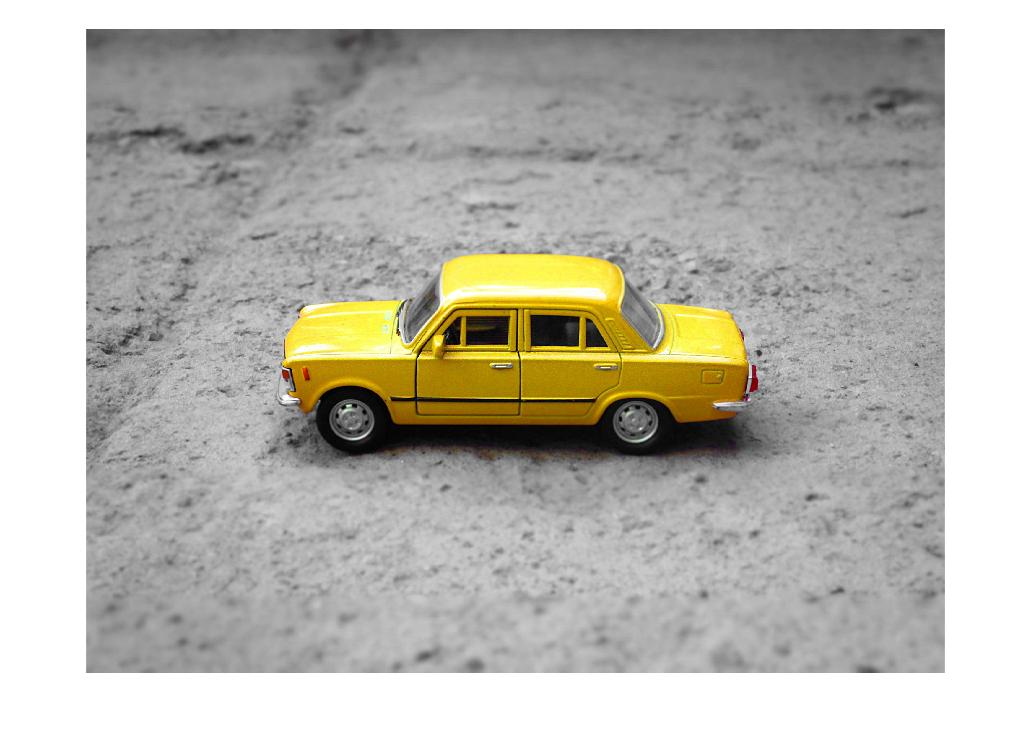
\includegraphics[width=220pt]{toyCar}
      		\caption{Image by Gustavo, Upsplash.}
		    \label{fig:toycarA}
    	\end{subfigure}%
    	\begin{subfigure}[b]{0.5\linewidth}
      		\centering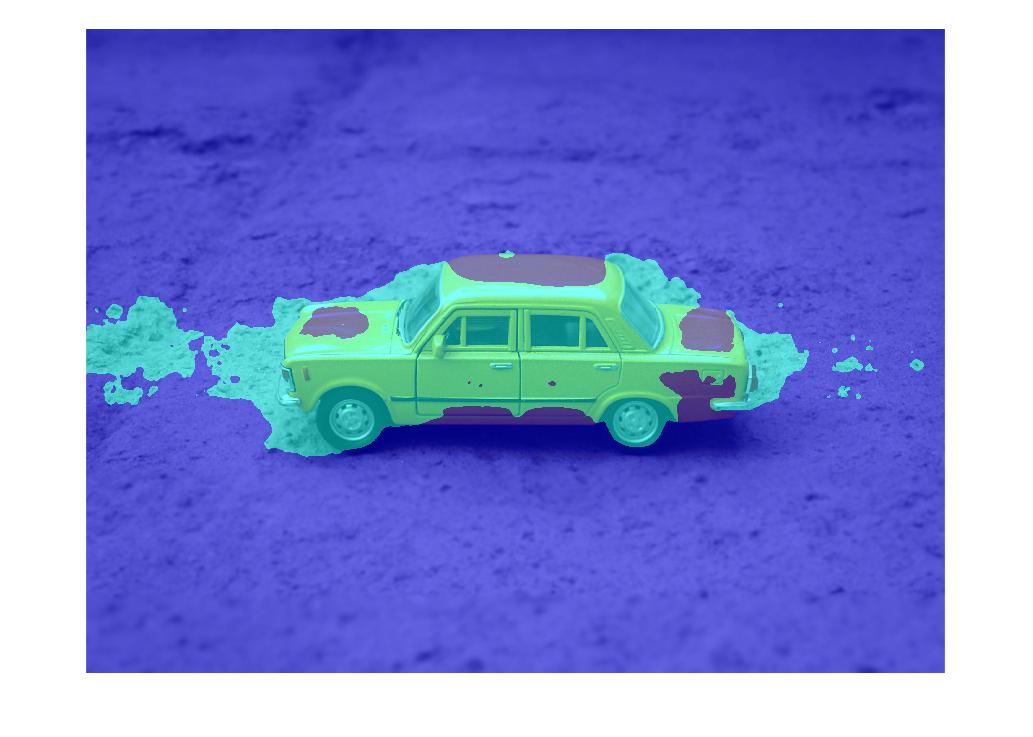
\includegraphics[width=220pt]{toycarseg}
      		\caption{Segmentation of car from background.}
       		\label{fig:toycarB}
    	\end{subfigure}
    	\caption{Segmentation of toy cars using K-Means Clustering.}
    	\label{fig:toycar}
\end{figure} 

\subsection{K-Means}
There are many methods by which to segment an image with clustering but K-Means is very popular for its simplicity and speed. K-means produces K clusters implemented as follows

    \begin{enumerate}
    \itemsep0em
        \item Place K points on the image randomly or with some educated guess. These points are the initial centroids for the K clusters.  
        \item Assign all data points to their nearest centroid.
        \item Update the centroids' positions as the mean of all data points in that class.
        \item Repeat steps 2 and 3 until cluster centroids no longer move (converge). 
    \end{enumerate}

K-means is guided by trying to limit the variance within each class. Variance is described by the expression

\begin{equation}\label{eq:2}
   V = \sum_{i=1}^k\sum_{x_j\in c_i}(x_j-\mu_i)^2 
\end{equation}

Where {$x_j$} are the data vectors, $c_i$ are the classes that the data point belong to and $\mu_i$ are the class centroids.

Because the K-Means algorithm is fast and the success of the segmentation depends on the initial placement of centroids, often the algorithm is performed many times with different initial conditions and the instance that yields the best results is used. 


[ SHOW EXAMPLE OF K-MEANS CLUSTERING BEING USED ]